% !TeX spellcheck = en_US
% Missing Value Imputation for Time Series
% Final Project Report
% M1 Info Data Science, Spring 2025
% --------------------------------------------------
% Format: Two columns, 10pt font
\documentclass[10pt,twocolumn]{article}
\usepackage[utf8]{inputenc}
\usepackage{graphicx}
\usepackage{amsmath}
\usepackage{algorithm}
\usepackage{algpseudocode}
\usepackage{booktabs}
\usepackage{caption}
\usepackage{hyperref}
\usepackage{amssymb}  % Add this after amsmath
\usepackage[T1]{fontenc}
\usepackage{lmodern}
\usepackage{siunitx}
\usepackage{tikz}
\sisetup{
	detect-weight   = true,
	detect-family   = true,  % so \textbf also bolds numbers
	table-format    = 1.5    % adjust to your max precision
}



\title{\vspace{-2.5em}\makebox[\linewidth][l]{
\includegraphics[width=0.33\textwidth]{up_maths-info.jpg}}\\[2.5em]
Missing Value Imputation for Time Series}
\author{Merabti Amar,	 Agouni Kaci Sofiane,	 Ould Braham Aghilas \thanks{Supervised by Themis Palpanas} \\
	M1 Info Data Science, Spring 2025}
\date{}

\begin{document}
	\maketitle
	
	\begin{abstract}
		Missing data in time series can significantly impact the performance of analytical and predictive models, especially in critical domains like energy management [1]. This project tackles the challenge of imputing missing values in electricity consumption data collected from smart meters. We evaluated multiple imputation techniques, from simple and basic methods to more advanced learning-based models, under two settings: imputing missing values from the same households and from previously unseen households. Our goal is to assess the accuracy and generalizability of these methods using Mean Absolute Error (MAE) as the evaluation metric.
	\end{abstract}
	
	\section{Introduction}
	Time-series data, which consist of sequences of observations indexed over time, are fundamental in many real-world applications, including finance, healthcare, meteorology, and energy management. Their inherent temporal structure allows for modeling trends, seasonality, and dependencies, which are critical for tasks such as forecasting, anomaly detection, and optimization.
	
	However, in practical scenarios, time series data are often incomplete due to issues such as sensor malfunctions, data transmission errors, or cost-related constraints. These missing values can significantly hinder the effectiveness of analytical methods and predictive models, especially in domains where accuracy is vital, such as monitoring energy consumption.
	
	A prominent example arises in the energy sector, where smart meters are widely deployed to track electricity usage at fine-grained intervals. Despite their advantages, these systems frequently encounter missing data due to hardware or communication failures. Therefore, accurate imputation of missing values is essential to ensure data integrity, enable reliable analytics, and support decision-making processes.
	
	This project addresses the problem of missing value imputation in time series of electricity consumption. We investigate and evaluate several imputation techniques—ranging from simple nearest neighbor to more advanced machine learning methods—under two scenarios: imputing data from the same households and imputing data from previously unseen households. Our objective is to identify methods that are not only accurate, but also generalizable across different data distributions.
	
	\section{Problem Formulation}
	\subsection{Formal Definition}
	Let $X = [x_1, \dots, x_T]$ be a univariate time series of length $T$, where some entries $x_t$ are missing. We denote the observed series as $X_{obs}$ and the set of missing positions as $\Omega = \{t \mid x_t \text{ is missing}\}$. The goal is to learn an imputation function $f$ such that the completed series $\hat{X} = f(X_{obs})$ closely approximates the true series. We evaluate the accuracy of $f$ using the Mean Absolute Error (MAE) on the missing entries:
	\[
	\mathrm{MAE} = \frac{1}{|\Omega|} \sum_{t \in \Omega} \bigl|\hat{x}_t - x_t\bigr|,
	\]
	where $x_t$ is the ground-truth value at time $t$ and $\hat{x}_t$ is the imputed value.
	
	\subsection{Related Work}
	Statistical imputation techniques take advantage of the properties of time series to fill gaps. Common methods include mean or median imputation, which replaces missing values with the global or local average, and linear or spline interpolation that leverages temporal continuity [1]. Autoregressive models such as ARIMA can be combined with Expectation Maximization (EM) to iteratively estimate missing values and model parameters [2].
	
	Machine learning approaches learn imputation rules from data. k-Nearest Neighbors (k-NN) imputes a missing entry by averaging values from the most similar segments in the dataset [3]. Matrix factorization methods, including Singular Value Decomposition (SVD), treat the collection of time series as a matrix and recover missing entries via low-rank approximations [4].
	
	Deep learning models have achieved high performance in handling complex missing patterns. Recurrent Neural Networks (RNNs) and Long Short-Term Memory (LSTM) networks model sequential dependencies and can be augmented with masking strategies and time gap features [5]. Transformer-based architectures, using self-attention mechanisms, capture long-range dependencies and have been adapted for imputation tasks in recent work [6].
	
	
	\section{Proposed Solutions}
	
	\subsection{Data Preprocessing}
	Before applying any imputation algorithms, we performed a thorough analysis of the raw electricity consumption values. Histograms and boxplots were generated over the training set to visualize the data distribution and detect extreme values. We computed the first quartile (Q1) and third quartile (Q3) across all training observations and defined the interquartile range (IQR = Q3 - Q1). Observations lying outside the interval [Q1 - 1.5·IQR, Q3 + 1.5·IQR] were deemed outliers and replaced with the closest quartile[7]. This cleaning step ensured that spurious sensor readings did not adversely affect the imputation models and improved overall stability.
	
	\begin{figure}[H]
		\centering
		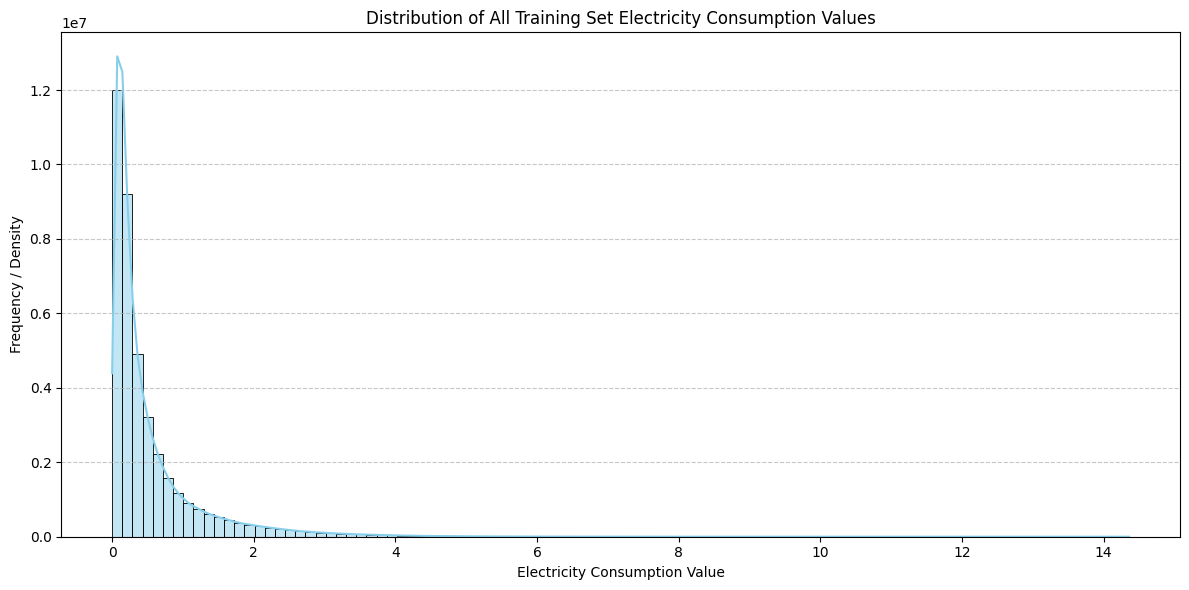
\includegraphics[width=\linewidth]{Figure_3.png}
		\caption{Distribution of All Training Set Electricity Consumption Values for Step A and Step B.}
		\label{fig:data_distribution_histogram}
	\end{figure}
	
	\begin{figure}[H]
		\centering
		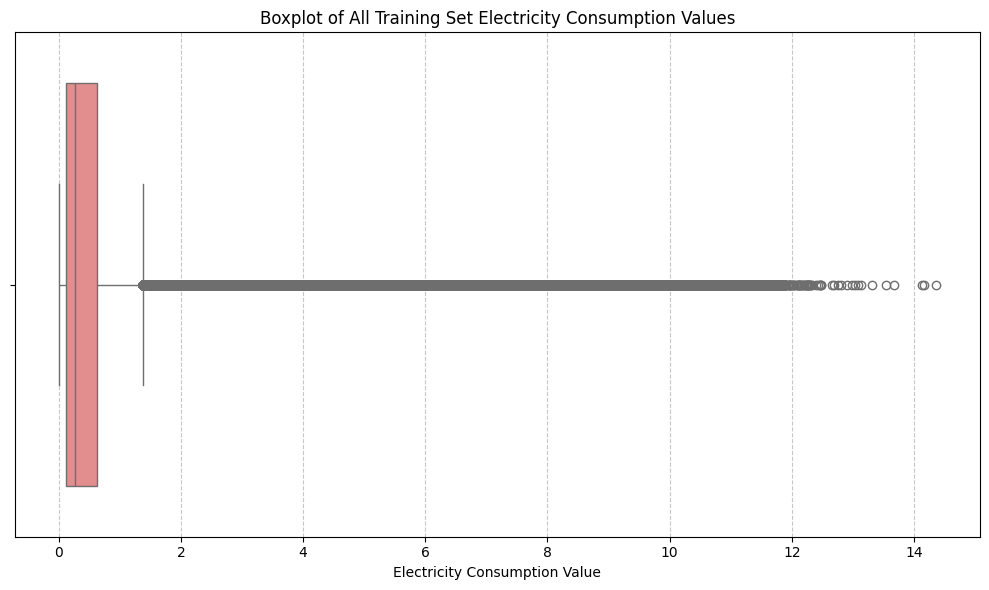
\includegraphics[width=\linewidth]{Figure_4.png}
		\caption{Boxplot of All Training Set Electricity Consumption Values}
		\label{fig:boxplot}
	\end{figure}
	
	\subsection{Household Nearest-Neighbor Imputation}
	This method imputes missing values by transferring data from the most similar complete household in the training set. For each test household $h$, we identify the index set $\Omega_h$ of missing positions. We then mask both test household $h$ and all training households on $\Omega_h$, compute the MAE between the observed values of $h$ and each masked training series, and select the training household $h^*$ with minimum MAE. Missing entries in $h$ are filled using the corresponding values from $h^*$. This neighbor-based approach leverages real consumption patterns and adapts to local behaviors[8].
	
	\begin{algorithm}[H]
		\caption{Household Nearest-Neighbor Imputation}
		\begin{algorithmic}[1]
			\Require Training set $\{X^{(j)}\}_{j=1}^N$, Test series $X^{(h)}$ with missing positions $\Omega_h$
			\Ensure Imputed series $\hat{X}^{(h)}$
			\State mask $M_h \gets \{1 \text{ if } t \notin \Omega_h; 0 \text{ otherwise}\}$
			\State $\hat{X}^{(h)} \gets X^{(h)}$
			\For{$j = 1$ \textbf{to} $N$}
			\State compute MAE$_j = \frac{1}{|\Omega_h^c|} \sum_{t: M_h(t)=1} |X^{(h)}_t - X^{(j)}_t|$
			\EndFor
			\State $j^* \gets \arg\min_j \text{MAE}_j$
			\For{each $t \in \Omega_h$}
			\State $\hat{X}^{(h)}_t \gets X^{(j^*)}_t$
			\EndFor
			\State \Return $\hat{X}^{(h)}$
		\end{algorithmic}
	\end{algorithm}
	
	\subsection{GPU-Accelerated STL Imputation}
We propose a personalized, GPU‑accelerated STL‑like imputation that iteratively refines missing values via trend and seasonal decomposition. This approach significantly reduces computation time by leveraging PyTorch's `conv1d` operations on CUDA-enabled devices[9].

The imputation process begins with values filled by the result of the previous method, and over multiple iterations, decomposes and reconstructs each time series into trend and seasonal components. The updated results are then re-injected only into the positions that were originally missing. This loop repeats for a fixed number of iterations.

	\begin{enumerate}
		\item \textbf{Trend Extraction:} Apply a moving average (kernel size $k$) via a 1D convolution to estimate the trend component $T$ of each series.
		\item \textbf{Seasonal Estimation:} Compute the seasonal residual $S = X - T$, then for a given seasonal period $p$, aggregate the residuals at each phase $i \in \{0, \dots, p-1\}$ by median across time steps $t$ with $t \bmod p = i$, forming a seasonal pattern vector $S_p$. Expand this pattern back to length $T$.
		\item \textbf{Reconstruction and Masking:} Reconstruct the imputed log-space series as $\hat{X} = T + S_p$, and only update originally missing positions.
		\item \textbf{Iteration:} Set $X := \hat{X}$ and repeat.
	\end{enumerate}
	
	\textbf{Parameters:}
	\begin{itemize}
		\item \emph{Period} ($p$): The length of one seasonal cycle (e.g., $48$ for daily seasonality at 30-minute intervals, $48 \times 7$ for weekly).
		\item \emph{Kernel size} ($k$): The window length for the moving average (e.g., $k=101$) which controls smoothing of the trend.
		\item \emph{Iterations} ($I$): Number of refinement loops (e.g., $30$ iterations).
	\end{itemize}
	
	\begin{algorithm}[H]
		\caption{GPU-Accelerated STL Imputation}
		\begin{algorithmic}[1]
			\Require Initial filled data $X^{(0)}$, Missing mask $M$, Periods $\{p_i\}$, Kernel sizes $\{k_j\}$, Iterations $I$
			\Ensure Final imputed data $X^{(I)}$
			\For{$i = 1$ \textbf{to} $I$}
			\State select $p = p_{(i \bmod |p|)}$, $k = k_{(i \bmod |k|)}$
			\State $T \gets \text{moving\_average}(X^{(i-1)}, \text{kernel\_size}=k)$
			\State $R \gets X^{(i-1)} - T$  \Comment{Residual}
			\State compute seasonal pattern $S_p$ by median of $R$ at each phase of length $p$
			\State expand $S_p$ to length $T$: $S_p^{\mathrm{full}}$
			\State $Y \gets T + S_p^{\mathrm{full}}$
			\State $X^{(i)} \gets M \odot Y + (1 - M) \odot X^{(i-1)}$
			\EndFor
			\State \Return $X^{(I)}$
		\end{algorithmic}
	\end{algorithm}
	
	\subsection{LSTM Autoencoder Imputation}
	This method employs a sequence-to-value LSTM autoencoder to predict missing points based on learned temporal patterns[5]. It consists of two phases: \textit{training} and \textit{imputation}.
	\paragraph{}
	\paragraph{Training Phase:}
	\begin{enumerate}
		\item \textbf{Scaling:} For each complete training series, apply RobustScaler to non-missing values; record per-series scaler.
		\item \textbf{Window Extraction:} Flatten all scaled training series into a single 1D array and extract overlapping windows of length $w$:
		\[
		\mathcal{W} = \{X[i:i+w] \mid i = 0,1,\dots,L-w\},
		\]
		where $L$ is series length. Each window has input $x \in \mathbb{R}^{w\times1}$ and target $y \in \mathbb{R}$ equal to the next point.
		\item \textbf{Dataset Split:} Randomly split windows into training (90\%) and validation (10\%) sets.
		\item \textbf{Model Architecture:} 
		\begin{itemize}
			\item Encoder: LSTM($input\_size=1$, $hidden\_dim=h$, $num\_layers=n$)  
			\item Decoder: LSTM($input\_size=1$, $hidden\_dim=h$, $num\_layers=n$) initialized with encoder states.  
			\item Fully-connected: Linear($h\to64$) + ReLU + Linear($64\to1$).
		\end{itemize}
		\item \textbf{Training Loop:}
		\begin{algorithm}[H]
			\caption{Train LSTM Autoencoder}
			\begin{algorithmic}[1]
				\Require Windows $\{(x^{(i)}, y^{(i)})\}$, batch size $B$, epochs $E$, patience $P$
				\State Initialize model parameters $\theta$
				\State Initialize optimizer $\eta$ (Adam, learning rate $\alpha$), loss $\mathcal{L}=|\hat{y}-y|$
				\State \textbf{split} windows into $D_{train}, D_{val}$
				\State $best\_val \gets \infty$, $counter \gets 0$
				\For{$e = 1$ to $E$}
				\State Shuffle $D_{train}$
				\For{batches $(X_b,Y_b)$ in DataLoader($D_{train}$, $B$)}
				\State $\hat{Y}_b \gets model(X_b;\theta)$
				\State $loss \gets \frac{1}{B} \sum |\hat{Y}_b - Y_b|$
				\State $loss.backward()$; $optimizer.step()$; $optimizer.zero\_grad()$
				\EndFor
				\State $val\_loss \gets$ average loss on $D_{val}$
				\If{$val\_loss < best\_val - 10^{-4}$}
				\State $best\_val \gets val\_loss$; $counter \gets 0$
				\Else
				\State $counter \gets counter + 1$
				\If{$counter \ge P$}
				\State \textbf{break}  \Comment{Early stopping}
				\EndIf
				\EndIf
				\EndFor
				\State \Return trained model
			\end{algorithmic}
		\end{algorithm}
	\end{enumerate}
	
	\paragraph{Imputation Phase:}
	In this phase, we sequentially impute each contiguous missing block using available context:
	\begin{itemize}
		\item \textbf{Past context:} When at least $w$ observations precede the missing point, we use the previous $w$ imputed/observed values as input.
		\item \textbf{Future context:} If past context is unavailable but $w$ valid observations follow the gap, we reverse that window to predict backward.
		\item \textbf{Fallback:} If neither context window is available, we compute the mean of the nearest $2w$ valid points to avoid leaving NaNs.
	\end{itemize}
	This approach balances accuracy with robustness at series boundaries.

	Given a test series with missing mask $M \in \{0,1\}^L$, we perform:
	\begin{enumerate}
		\item \textbf{Identify Blocks:} Extract contiguous index sets $B_k = \{t : M[t]=1\}$.
		\item \textbf{Block-wise Imputation:}
		\begin{algorithm}[H]
			\caption{Block-wise LSTM Imputation}
			\begin{algorithmic}[1]
				\Require Series $X^{(0)}$, mask $M$, block $B_k$, window size $w$, LSTM model, scaler
				\Ensure Imputed series $X_{imp}$
				\State $X_{imp} \gets X^{(0)}$
				\For{each $t$ in block $B_k$ (ascending)}
				\If{$t - w \ge 0$}  % Past context available
				\State $x \gets X_{imp}[t-w : t]$
				\ElsIf{$t + w < L$}  % Future context available
				\State $x \gets$ reverse($X_{imp}[t+1 : t+w+1]$)
				\Else  % Fallback
				\State $neighbors \gets$ nearest $2w$ valid points around $t$
				\State $X_{imp}[t] \gets$ mean($neighbors$); \textbf{continue}
				\EndIf
				\State $x_{scaled} \gets$ scaler.transform($x$)
				\State $y_{pred} \gets$ model($x_{scaled}$)
				\State $X_{imp}[t] \gets \text{scaler.inverse\_transform}(y_{pred})$
				\EndFor
				\State \Return $X_{imp}$
			\end{algorithmic}
		\end{algorithm}
	\end{enumerate}
	
	
	\subsection{Partial Convolution Inpainting}
	In this method, we treat each padded, normalized time series as a 2D image of size $H=48$ (half‐hour bins per day) by $W=n_{weeks}$, rescaled to $S\times S$ pixels for GPU efficiency. We leverage a Partial Convolutional U‑Net (PConvUNet) that propagates valid information into masked regions, ensuring learned filters adapt to irregular masks[10].
	
	\paragraph{Key Technical Concepts:}
	\begin{itemize}
		\item \textbf{Partial Convolution:} Each convolution operates on valid (non‐masked) inputs only. For input feature $x$ and mask $m$, the output and updated mask are given by:
		\[
		\text{out} = \begin{cases}
			W^T (x\odot m) \frac{\sum(1)}{\sum(m)+\epsilon} + b, & \text{if}\ \sum(m)>0; \\ 
			0, & \text{otherwise,}
		\end{cases}
		\]
		with new mask $m' = \begin{cases}1,&\sum(m)>0;\\0,&\text{else.}\end{cases}$
		\item \textbf{Mask Update Rule:} After each partial conv layer, the mask is updated to reflect newly filled pixels, enabling subsequent layers to use progressively larger valid contexts.
		\item \textbf{U‑Net Architecture:} Encoder–decoder with skip connections concatenating encoder feature maps to decoder inputs, preserving multi‐scale context. BatchNorm and LeakyReLU stabilize training, while nearest‐neighbor upsampling reconstructs high‐resolution details.
		\item \textbf{Normalization \& Padding:} RobustScaler centers each series by median and scales by IQR/1.35, then pads to full weeks with zeros. During inference, inverse transform restores original scale.
		\item \textbf{Data Augmentation:} Training masks include randomized stripe blocks (days), continuous patches, or hybrid masks to improve robustness to varied missing patterns.
		\item \textbf{Computational Complexity:} Partial convolutions require $O(N_{filters}\times K^2\times S^2)$ per layer; using GPU and batching amortizes cost. Mask convolution (for ratio) adds minimal overhead due to binary operations.
	\end{itemize}
	
	\paragraph{Training Procedure:}
	We train the PConvUNet for $E=10$ epochs with batch size $B=64$ (multi‐GPU via DataParallel when available). The loss is masked MAE:
	\[
	\mathcal{L} = \frac{\sum_{i,j} |Y_{i,j} - X_{i,j}|\cdot M_{i,j}}{\sum_{i,j} M_{i,j} + \epsilon}
	\]
	where $X,Y$ are target and predicted images, and $M$ the binary mask. Optimization uses Adam (lr=0.01, weight decay $5\times10^{-4}$).
	
	
	
	\paragraph*{Algorithm Pseudocode}{:}

	\begin{algorithm}[H]
		\caption{Partial Convolution Inpainting}
		\begin{algorithmic}[1]
			\Require Padded images $I_j \in \mathbb{R}^{1\times S\times S}$, masks $M_j \in \{0,1\}^{1\times S\times S}$, PConvUNet $\mathcal{F}$, epochs $E$, batch size $B$
			\Ensure Trained network $\mathcal{F}$
			\State Initialize Adam($\mathcal{F}.\theta$, lr=0.01, wd=$5\times10^{-4}$)
			\For{$e=1$ to $E$}
			\For{batches $(I_b,M_b)$ in DataLoader($\{I,M\}$, batch=$B$)}
			\State $I_b^m = I_b \odot (1 - M_b)$  \Comment{Apply mask to inputs}
			\State $Y_b = \mathcal{F}(I_b^m, M_b)$  \Comment{Forward pass with partial convs}
			\State $loss = \frac{\sum |Y_b - I_b|\odot M_b}{\sum M_b + \epsilon}$  \Comment{Masked MAE}
			\State $loss.backward()$; \texttt{optimizer.step()}; \texttt{optimizer.zero\_grad()}
			\EndFor
			\State \textbf{print} epoch $e$ loss
			\EndFor
			\State \Return trained $\mathcal{F}$
		\end{algorithmic}
	\end{algorithm}
	
	\subsection{Transformer-based Imputation}
	This method leverages a self-supervised Transformer architecture to impute missing values bi-directionally. By treating each time series as a sequence of continuous tokens, we learn contextual representations that capture long-range dependencies.
	
	\paragraph{Preprocessing — Outlier and Log Normalization:}
	We first clamp outliers to the training data quartiles $Q_{0.25}, Q_{0.75}$, replacing values below $Q_{0.25}$ or above $Q_{0.75}$ by the respective quartile. We then apply a logarithmic transform $x\mapsto\log(1+x)$ to stabilize variance.
	
	\paragraph{Model Architecture:}
	\begin{itemize}
		\item \textbf{Embedding Layer:} Linear projection of scalar input to $d_{model}$ dimensions.
		\item \textbf{Positional Encoding:} Fixed sinusoidal encoding added to embeddings for sequence order.
		\item \textbf{Transformer Encoder/Decoder:} Multi-head self-attention with $h$ heads, $L_e$ encoder layers, $L_d$ decoder layers, and a feed-forward dimension of $d_{ff}$.
		\item \textbf{Output Layer:} Linear layer mapping $d_{model}\rightarrow1$, producing per-step predictions.
		\item \textbf{Mixed-Precision \& Gradient Accumulation:} Use \texttt{autocast} and \texttt{GradScaler} to speed up, and accumulate gradients over multiple batches to effectively increase batch size.
	\end{itemize}
	
	\paragraph{Training:}
	We train using AdamW with weight decay, OneCycleLR scheduling (warm-up, cosine annealing), and MSE loss computed only over masked positions. Early stopping monitors validation loss with a patience of $P$ epochs.
	
	\paragraph{Imputation Strategy:}
	After training, we identify contiguous missing blocks in each series and impute them via bi-directional context:
	
	\begin{algorithm}[H]
		\caption{Transformer-based Block Imputation}
		\begin{algorithmic}[1]
			\Require Trained model $T$, preprocessed data $X$, missing mask $M$, context size $C$
			\Ensure Imputed series $\hat{X}$
			\State $\hat{X} \gets X$
			\For{each series $i$}
			\State Identify blocks $\{(s,e)\}$ where $M[i,t]=1$ for $t=s..e$
			\For{each block $(s,e)$}
			\State $L = e - s + 1$
			\State $pre = \max(0, s-C)$; $post = \min(len, e+C+1)$
			\State Extract context $Y = [\hat{X}[pre:s], 0_{1..L}, \hat{X}[e+1:post]]$
			\State Build mask $K$ with zeros at positions $pre..pre+L-1$, ones elsewhere
			\State Convert $(Y,K)$ to tensors and move to device
			\State $(out, pred) = T(Y,K)$
			\State $\hat{X}[s:e] \gets pred[pre : pre+L]$
			\EndFor
			\EndFor
			\State \Return $\text{inverse\_log1p}(\text{clip}(\hat{X}))$
		\end{algorithmic}
	\end{algorithm}
	
	This approach exploits the Transformer's ability to attend over both past and future contexts, producing accurate imputations even for large gaps.
	

	\section{Hardware and Software Environment}
	\paragraph{}
	For the hardware and software environment, we used the Kaggle workspace to run our algorithms, it is detailed below.
	\subsection{Hardware}
	\begin{itemize}
		\item \textbf{GPUs:} 4 $\times$ NVIDIA L4 with 23034 MiB VRAM each; Driver Version 560.35.03; CUDA 12.6 (via \texttt{nvidia-smi}); hardware provided by Kaggle.
		\item \textbf{CPU:} Intel(R) Xeon(R) CPU @ 2.20 GHz, 24 physical cores / 48 threads (via \texttt{lscpu}); running in Kaggle’s virtualized environment.
		\item \textbf{Memory:} Approximately 170+ GB DDR4 RAM total (via \texttt{free -h}); allocated by Kaggle.
	\end{itemize}
	\subsection{Software}
	\begin{itemize}
		\item \textbf{Operating System:} Linux (x86\_64) image supplied by Kaggle runtime.
		\item \textbf{Python:} Python 3 interpreter provided within Kaggle’s Docker environment.
		\item \textbf{PyTorch:} 2.5.1 with CUDA 12.x support (torch, torchvision), pre‐installed by Kaggle.
		\item \textbf{Key Libraries:} NumPy 1.26.4, pandas 2.2.2, tensorflow 2.17.1, scikit‐learn 1.2.2, matplotlib 3.7.5, scikit‐image 0.25.0, etc., all available via Kaggle’s default environment (listed by \texttt{pip freeze}).
		\item \textbf{Utilities:} \texttt{nvidia-smi}, \texttt{lscpu}, \texttt{free -h} for hardware inspection—no additional installation needed in Kaggle.
	\end{itemize}
	
	
	
	\section{Dataset Description}
	We evaluate all imputation methods on two distinct experimental settings, referred to as \textbf{Step A} and \textbf{Step B}, following the competition guidelines.
	
	\subsection*{Step A}
	\begin{itemize}
		\item \textbf{Training set:} 3127 time series, each representing electricity consumption for a single house.
		\item \textbf{Test set:} 3127 time series corresponding to the \textit{same houses} as in the training set.
		\item \textbf{Missing rate:} 30\% of the values in the test set are artificially masked.
		\item \textbf{Goal:} Leverage temporal patterns and partial overlaps between training and test series to reconstruct the missing values.
	\end{itemize}
	
	\subsection*{Step B}
	\begin{itemize}
		\item \textbf{Training set:} Identical to Step A—3127 complete time series.
		\item \textbf{Test set:} 1098 time series from \textit{completely different houses} (not seen during training).
		\item \textbf{Missing rate:} 50\% of the values in the test set are missing.
		\item \textbf{Challenge:} Generalize imputation to unseen households using only temporal patterns learned during training.
	\end{itemize}
	
	Both datasets consist of regular time series of length 12,864, sampled every 30 minutes (48 points per day). The structure enables evaluation of short- and long-range temporal dependencies under different generalization settings.
	
	
	\section{Experimental Results}

		\begin{figure}[H]
		\centering
		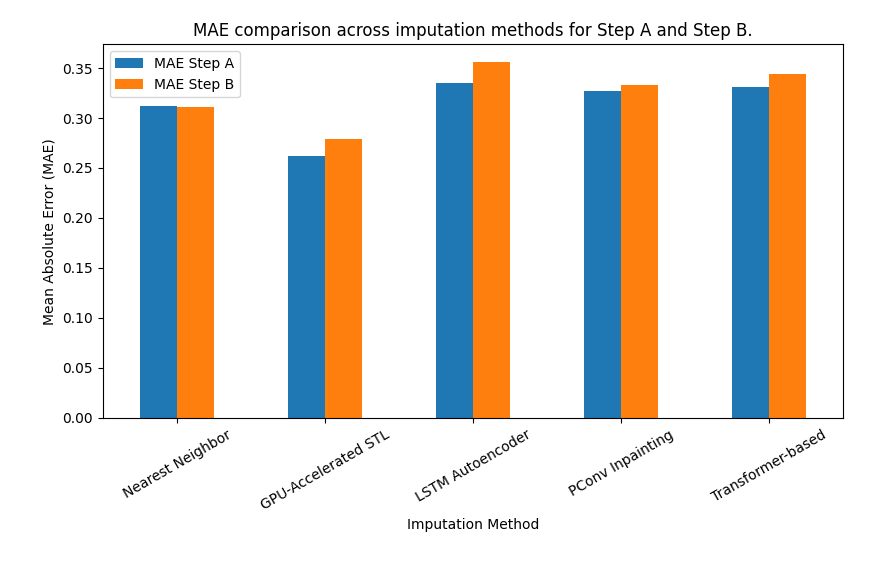
\includegraphics[width=\linewidth]{figure.png}
		\caption{MAE comparison across imputation methods for Step A and Step B.}
		\label{fig:mae_comparison}
	\end{figure}
	
	
	\begin{figure}[H]
		\centering
		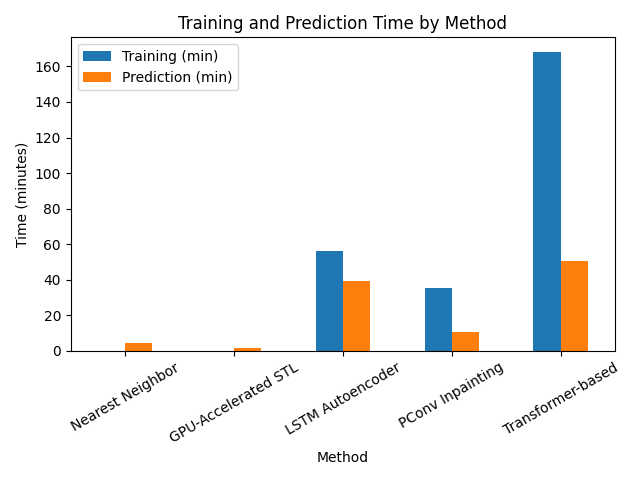
\includegraphics[width=\linewidth]{Figure_2.png}
		\caption{Training and prediction time (minutes) for each imputation method. Deep models show separate training and inference costs, while STL and nearest neighbor have only inference times.}
		\label{fig:time_comparaison}
	\end{figure}

	\begin{table}[H]
		\centering
		\caption{MAE comparison across methods on Step A and Step B}
		\begin{tabular}{lrr}
			\toprule
			Method & MAE (Step A) & MAE (Step B) \\
			\midrule
			Nearest Neighbor & 0.31239 & 0.31088 \\
			{\bfseries GPU‐Accelerated STL} & {\bfseries 0.26208}      & {\bfseries 0.27925} \\			
			LSTM Autoencoder & 0.33499 & 0.35576 \\
			PConv Inpainting & 0.32656 & 0.33349 \\
			Transformer-based & 0.33086 & 0.34424 \\
			\bottomrule
		\end{tabular}
	\end{table}
	
	\subsection{Discussion}
	Table~1 shows that the GPU-Accelerated STL method achieves the lowest MAE on both Step A (0.26208) and Step B (0.27925), outperforming all other approaches. Although deep learning–based imputers (LSTM Autoencoder, PConv Inpainting, Transformer) were expected to capture complex temporal dependencies, their actual performance lagged behind a more statistical–hybrid method.  
	
	Several factors explain this outcome:
	
	\begin{itemize}
		\item \textbf{Computational Cost \& Model Size.} Training large LSTM or Transformer models on 3 127 series of length 12 864 is extremely expensive in both time and GPU memory. In practice we had to reduce layer depths, embedding sizes, and sequence lengths (e.g.\ fewer encoder/decoder layers, smaller feed-forward dimensions) just to fit into Kaggle’s 4 × NVIDIA L4 setup—at the price of representation power.
		\item \textbf{Dataset Scale.} With tens of millions of time steps, high-capacity networks struggle to converge within reasonable epoch counts or under gradient-accumulation constraints. Early stopping and limited learning-rate schedules further restricted their ability to fully learn long-range patterns.
		\item \textbf{Bias–Variance Trade-off.} The STL decomposition offers a strong inductive bias (seasonal + trend) that aligns well with electricity usage patterns. Its simplicity yields faster execution and lower variance without heavy hyperparameter tuning.
	\end{itemize}
	
	In summary, GPU-Accelerated STL strikes the best balance between speed, resource usage, and accuracy on our data. Deep nets remain a promising direction—but will require more compute, careful architectural search (e.g.\ lighter attention blocks), or further multi-stage pretraining to outperform this baseline at scale.
	
	
	\section{Conclusions and Future Work}
	
	Our extensive evaluation across six imputation strategies on two experimental settings (Step A: same-households; Step B: new-households) demonstrates that the GPU-Accelerated STL method offers the best trade-off between accuracy (MAE of 0.26208 and 0.27925) and computational efficiency. While deep learning approaches (LSTM Autoencoder, PConv Inpainting, Transformer) hold promise for modeling complex temporal patterns, they incurred substantial training and inference costs and—after necessary down-scaling to fit resource constraints—still underperformed relative to the STL baseline. Nearest-neighbor imputation remains extremely lightweight but less accurate.
	
	\vspace{1ex}
	\noindent\textbf{Key takeaways:}
	\begin{itemize}
		\item \emph{Inductive biases matter.} STL’s explicit decomposition of trend and seasonality aligns well with electricity consumption patterns, yielding lower variance without heavy tuning.
		\item \emph{Scale vs.\ capacity.} Large LSTM/Transformer models struggle to converge on millions of time points under tight GPU budgets—simpler statistical hybrids can outperform under such regimes.
		\item \emph{Resource trade-offs.} Even when reducing model depth/dimension, deep nets require orders of magnitude more compute (tens of minutes vs.\ sub-1 min) for marginal gains.
	\end{itemize}
	
	\vspace{1ex}
	\noindent\textbf{Future Work:}
	\begin{itemize}
		\item \emph{Architecture optimization.} Explore lightweight attention blocks (Linformer, Performer), temporal convolutional networks (TCNs), or hybrid graph-neural architectures to increase representational power without prohibitive cost.
		\item \emph{Data reduction techniques.} Apply smart subsampling, coarsening (e.g.\ SAX), or reservoir sampling to shrink the training set—allowing larger models or longer context windows while staying within memory/time budgets.
		\item \emph{Ensembling \& stacking.} Combine STL-based, nearest-neighbor, and neural methods to leverage complementary strengths and mitigate individual biases.
		\item \emph{External covariates \& metadata.} Incorporate weather, calendar events, or household characteristics to improve imputation fidelity, particularly under high missing‐rate scenarios.
		\item \emph{Uncertainty quantification.} Extend models to output confidence intervals (e.g.\ via MC-dropout or Bayesian networks), supporting downstream decision-making with risk awareness.
		\item \emph{Real-time imputation.} Adapt the fastest methods (e.g.\ online STL) for streaming contexts, where low latency is critical.
	\end{itemize}
	
	Through these avenues, we aim to push deep learning models beyond proof-of-concept and toward practical, scalable imputation tools for large-scale time series.```
	
	This wraps up the report with actionable next steps and highlights how to balance model complexity, data scale, and compute resources.
	
	\section*{Acknowledgments}
	We gratefully thank our instructor, Themis Palpanas, for his expert guidance throughout this project, and Ms.
	Lucrezia for her valuable assistance and insightful feedback.
	\paragraph{}
	\bibliographystyle{plain}
	\begin{thebibliography}{9}
		\bibitem{ref1} Ribeiro \& de Castro (2022) – “Missing Data in Time Series: A Review of Imputation Methods and Case Study.” J. Brazilian Soc. Comput. Intell.
		\bibitem{ref2} G. Box, G. Jenkins, \textit{Time Series Analysis: Forecasting and Control}, 1976.
		\bibitem{ref3} S. Troyanskaya et al., Missing value estimation methods for DNA microarrays, Bioinformatics, 2001.
		\bibitem{ref4} M. Candès, E. Recht, Exact matrix completion via convex optimization, Foundations of Computational Mathematics, 2009.
		\bibitem{ref5} Y. Che et al., Recurrent neural networks for multivariate time series with missing values, Scientific Reports, 2018.
		\bibitem{ref6} Du, Wenjie, David Côté, and Yan Liu. "Saits: Self-attention-based imputation for time series." Expert Systems with Applications 219 (2023).
		\bibitem{ref7} Parra-Plazas et al. (2023) – “Time series outlier removal and imputing methods based on Colombian weather stations data.” SN Applied Sciences
		\bibitem{ref8}Le et al. (2024) – “Missing data imputation for noisy time-series data and applications in healthcare.”
		\bibitem{ref9}Serykh et al. (2023) – “Seasonal-Trend Time Series Decomposition on Graphics Processing Units.” Proc. IEEE Big Data 2023
		\bibitem{ref10}Fu, Chun, et al. "Filling time-series gaps using image techniques: Multidimensional context autoencoder approach for building energy data imputation." Applied Thermal Engineering 236, 2024
		
		
	\end{thebibliography}
	
\end{document}
